%http://www.cmap.polytechnique.fr/~allaire/map411/MiniProjets/sujets2016/sujet_Augier.pdf

% --------------------------------------------------------------
%                         Template
% --------------------------------------------------------------

\documentclass[12pt]{article} %draft = show box warnings
\usepackage[utf8]{inputenc} % Accept different input encodings [utf8]
\usepackage[T1]{fontenc}    % Standard package for selecting font encodings
\usepackage{lmodern} % Good looking T1 font
\usepackage[a4paper, total={6.5in,10.2in}]{geometry} % Flexible and complete interface to document dimensions
\renewcommand{\baselinestretch}{1.0}

% --------------------------------------------------------------
%                         Other Fonts
% --------------------------------------------------------------
%\usepackage{mathpazo} % Hermann Zapf's Palatino font
%\usepackage{kpfonts} % Kepler font
%\usepackage{mathptmx} % Times New Roman Like Font
%\usepackage{eulervm} %  AMS Euler (eulervm) math font.

% --------------------------------------------------------------
%                         Package
% --------------------------------------------------------------
\usepackage[french]{babel} % Multilingual support [french]
\usepackage{enumerate} % Enumerate with redefinable labels
\usepackage{graphicx} % Enhanced support for graphics
\usepackage[makeroom]{cancel} % Place lines through maths formulae
\usepackage{booktabs} % Publication quality tables
\usepackage{braket} % Dirac bra-ket and set notations
\usepackage{epstopdf} % Convert EPS to ‘encapsulated’ PDF using Ghostscript
\usepackage{bbm} % "Blackboard-style" cm fonts
\RequirePackage{epsfig} % Include Encapsulated PostScript
\usepackage{float} % Improved interface for floating objects
\usepackage{amsmath,amsthm,amssymb} % American Mathematics Society facilities

\usepackage{stmaryrd} % St Mary Road symbols for theoretical computer science.
\usepackage{xfrac} % Create inline fraction
\usepackage{hyperref} % Create hyperf
\usepackage{secdot} % Put dots at the end of a section
\usepackage{comment}



%------------------- tikz --------------------------------------
\usepackage{tikz,bm,color}
\usetikzlibrary{shapes,arrows}
\usetikzlibrary{decorations}
\usetikzlibrary{decorations.pathreplacing,angles,quotes}
\usetikzlibrary{shapes.geometric,arrows,positioning}
\usetikzlibrary{calc}

% --------------------------------------------------------------
%                         Custom commands
% --------------------------------------------------------------
\newcommand*{\1}{\mathbbm{1}}
\newcommand*{\E}{\mathbb{E}}
\newcommand*{\Pb}{\mathbb{P}}
\newcommand*{\N}{\mathbb{N}} 
\newcommand*{\Z}{\mathbb{Z}}
\newcommand*{\car}{\text{card}}
\renewcommand*{\Re}{\operatorname{Re}}
\renewcommand*{\Im}{\operatorname{Im}}
\newcommand*\Laplace{\mathop{}\!\mathbin\bigtriangleup}
\newcommand*{\grad}{\nabla}
\renewcommand*{\O}{\mathcal{O}}

% --------------------------------------------------------------
%                         Exercise Environment
% --------------------------------------------------------------
\renewcommand{\thesection}{\Roman{section}}
\sectiondot{subsection}
\renewcommand{\subsubsection}{
	\pagebreak[2]
	\refstepcounter{subsubsection}
	\noindent
	\textbf{\thesubsubsection.}
}
% --------------------------------------------------------------

\begin{document}
	% --------------------------------------------------------------
	%                       Title  Header
	% --------------------------------------------------------------
	\noindent
	\normalsize\textbf{Approximation numérique et optimisation} \hfill \textbf{École Polytechnique}\\
	\normalsize\textbf{MAP 411} \hfill \textbf{\today}\vspace{20pt}
	\centerline{\Large Projet MAP411 – X2015}\vspace{5pt}
	\centerline{\Large \textbf{Applications de méthodes d'optimisation à la résolution des EDP}}\vspace{3pt}
	\centerline{Sujet proposé par Nicolas Augier -- \texttt{nicolas.augier@ens-cachan.fr}  }\vspace{13pt}
	\centerline{Lucas Lugão Guimarães -- \texttt{lucas.lugao-guimaraes@polytechnique.edu}  }
	\centerline{Alexandre Ribeiro João Macedo --  \texttt{alexandre.macedo@polytechnique.edu}}\vspace{20pt}
	% --------------------------------------------------------------
	
	\section{Méthodes de gradient}
	\subsection{Gradient à pas constant}
	\subsubsection{} %%I.1.1
	La figure \ref{fig:I11} montre les lignes de niveau de la fonction de Rosenbrock,
	\begin{align} \label{eq:rosenbrock}
	J(u_1,u_2)=(u_1-1)^2+100(u_1^2-u_2)^2 \text{,}
	\end{align}
	dans le rectangle $(u_1, u_2) \in [-1.5, 1.5] \textmd{ x } [0.5, 1.5]$.   
	\begin{figure}[ht]
		\begin{center}
    \hspace*{-1cm}  
	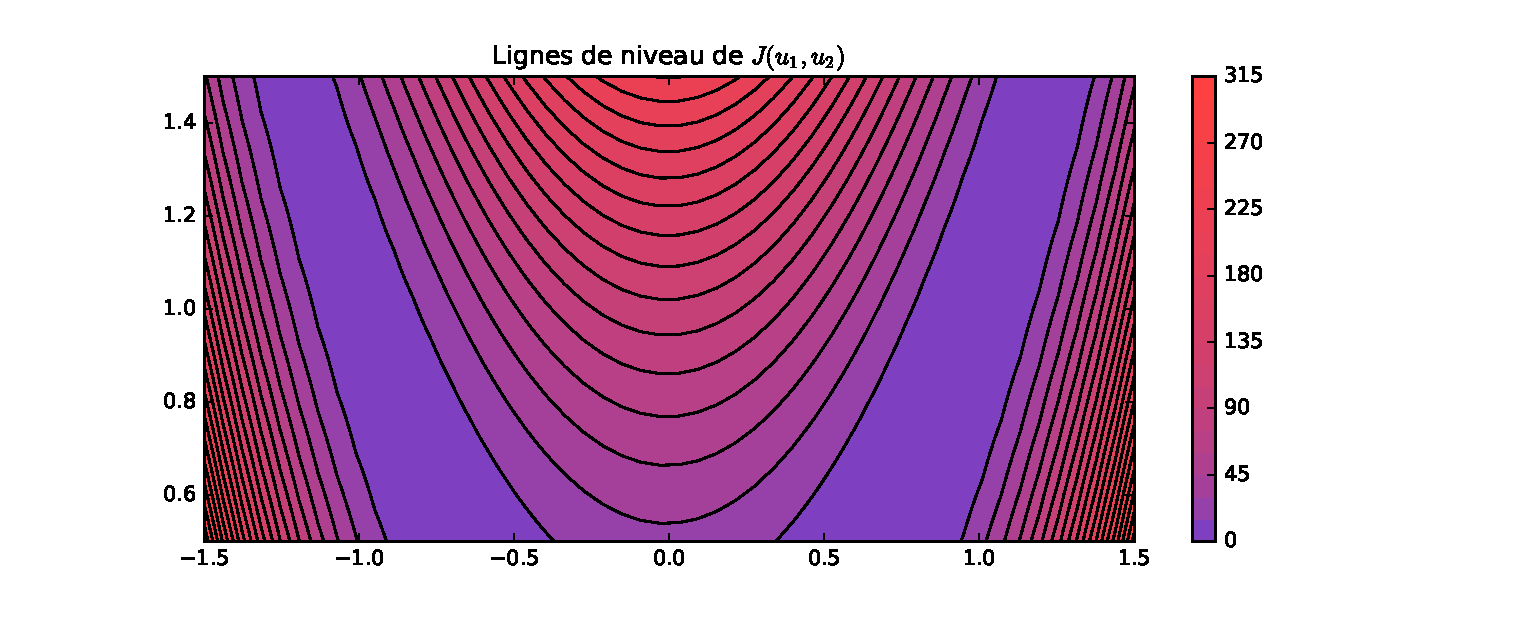
\includegraphics[height=8cm]{I11.eps}
        \vspace{-1cm}
		\end{center}
		\caption{Lignes de niveau de $J$.}
		\label{fig:I11}
	\end{figure}
	
	\subsubsection{} %% I.1.2
	On applique la méthode de gradient a pas constant $u_{k+1}=u_k-\rho \grad J(u_k)$ ou, pour $ u_k= (u_{k1},u_{k2})$, on a $\grad J(u_k) = ({400u_{k1}^3 + 2u_{k1}  - 400u_{k1}u_{k2} - 2}, {200u_{k1}^2 - 200u_{k2}})$. Pour les valeurs numériques $u_0=(1, 0)$ et $\rho = 0.002$, et le critère d'arrêt $J(u_{k+1}) < 10^{-3}$, on a besoin de \textbf{$12312$} itérations. La figure \ref{fig:I12} montre les lignes de niveau de l'équation \ref{eq:rosenbrock} et le parcours du méthode avant l'arrête.
	\begin{figure}[H]
		\begin{center}
	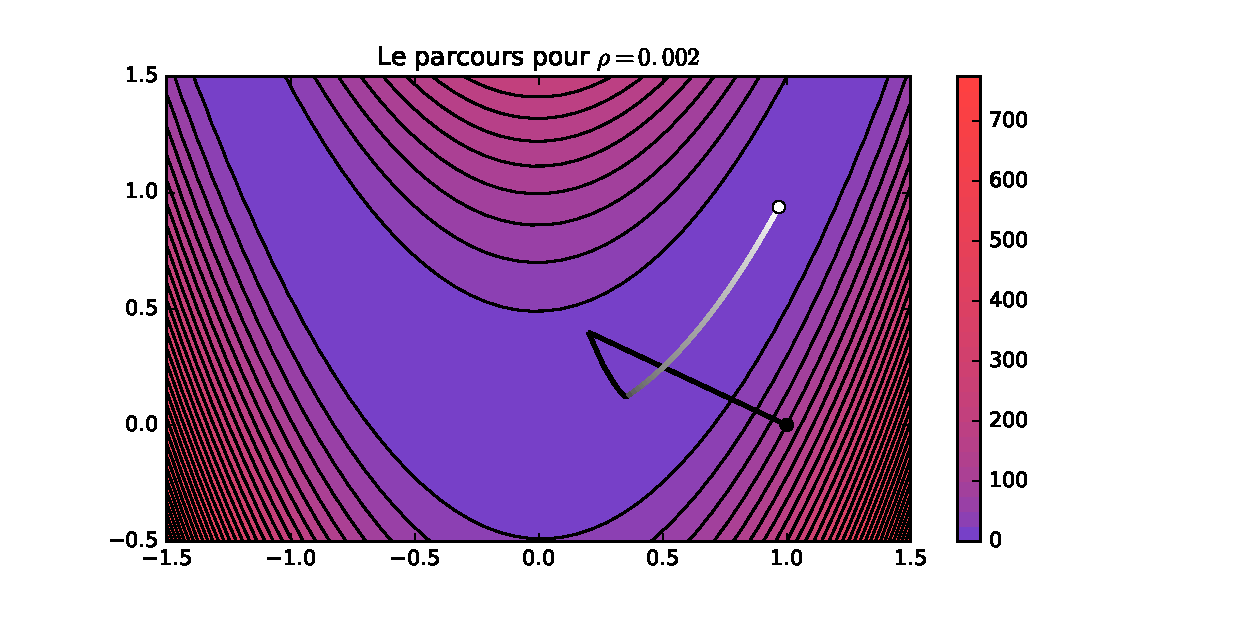
\includegraphics[height=8cm]{I12002.eps}
        \vspace{-1cm}
		\end{center}
		\caption{Parcours du méthode de gradient à pas constant.}
		\label{fig:I12p}
	\end{figure}
	
	\subsubsection{} %% I.1.3
	Si on applique le méthode pour $\rho = 0.0045$ et pour $\rho = 0.01$, on a que le méthode diverge. 
	\begin{figure}[H]
		\begin{center}
	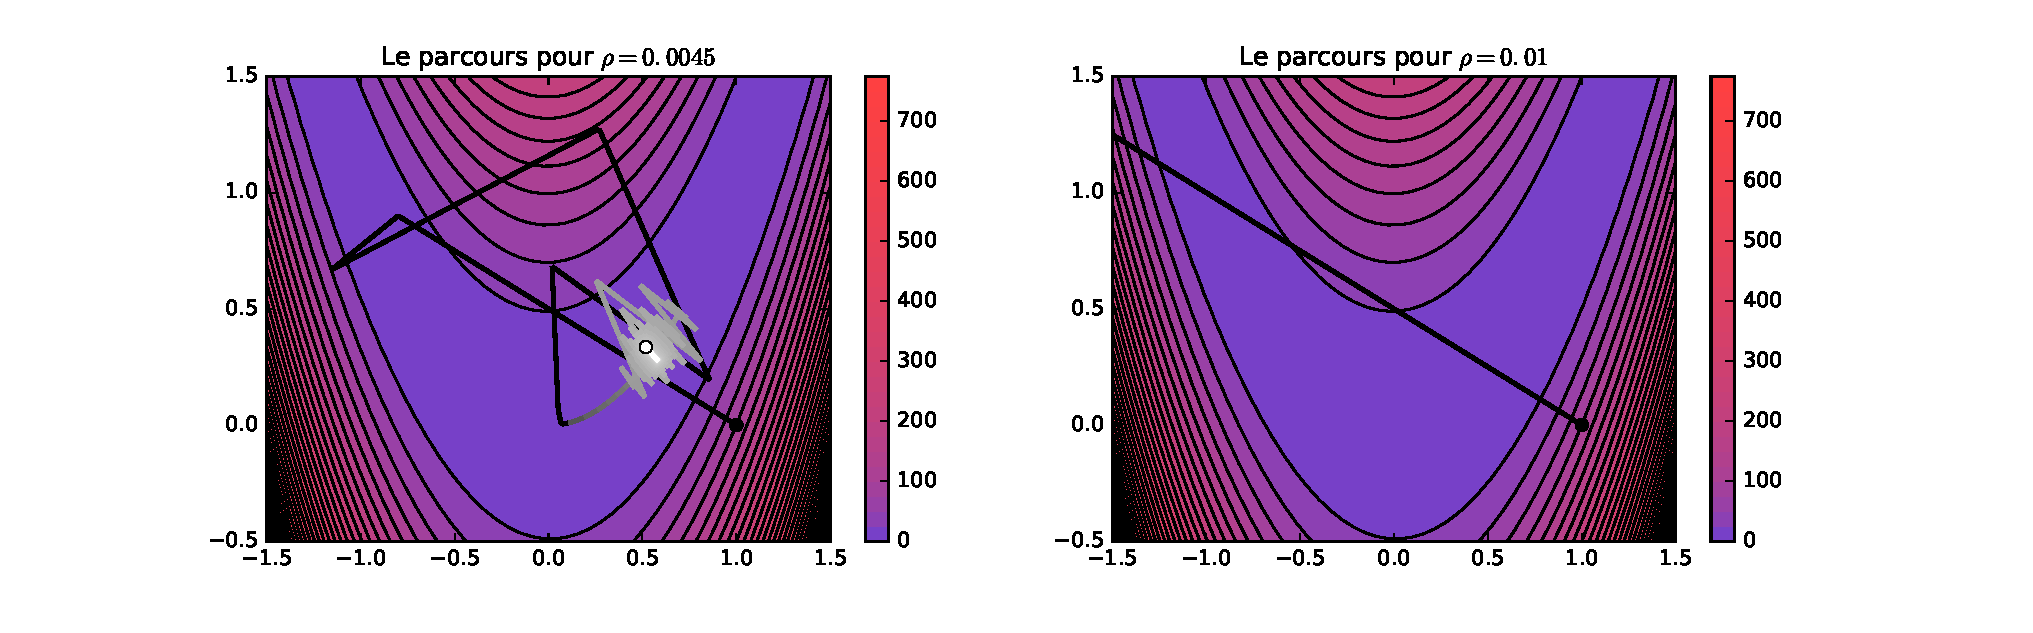
\includegraphics[height=5cm]{I12d.eps}
        \vspace{-1cm}
		\end{center}
		\caption{Le parcours du méthode de gradient à pas constant $\rho = 0.045$ et $\rho = 0.01$.}
		\label{fig:I12d}
	\end{figure}
    \newpage
	\subsection{Gradient optimal}
	\subsubsection{}
	Soit $J(u)=\frac{1}{2} \langle Au, u \rangle - \langle b, u \rangle$. On veut trouver ${\rho_k=\textrm{argmin}_{\rho \geq 0} J(u_k- \rho \grad J(u_k))}$. Soit ${r_k= \grad J(u_k) = Au_k-b}$, on a
	\begin{align} \label{eq:gradopt}
	\begin{split}
	J(u_k - \rho \grad J(u_k)) &= J(u_k - \rho r_k) \\ 
	&=  \frac{1}{2} \langle A(u_k - \rho r_k), u_k - \rho r_k \rangle - \langle b, u_k - \rho r_k \rangle \\
	&=\frac{1}{2} \langle Au_k, u_k \rangle - \langle b, u_k \rangle  + \frac{1}{2} \langle Au_k, - \rho r_k \rangle + \frac{1}{2} \langle - \rho A r_k, u_k \rangle + \frac{1}{2} \langle - \rho A r_k,  - \rho r_k \rangle  \\
	& \hphantom{==\frac{1}{2} \langle Au_k, u_k \rangle - \langle b, u_k \rangle  + \frac{1}{2} \langle Au_k, - \rho r_k \rangle + \frac{1}{2} \langle - \rho A r_k, u_k \rangle } - \langle b, - \rho r_k \rangle\\
    &= J(u_k) - \frac{\rho}{2} [\langle A u_k, r_k \rangle + \langle A r_k, u_k \rangle]+\frac{\rho^2}{2} \langle A r_k, r_k \rangle + \rho \langle b,  r_k \rangle \\
    &=J(u_k)  +\frac{\rho^2}{2} \langle A r_k, r_k \rangle + \rho [\langle b,  r_k \rangle -\langle A u_k, r_k \rangle] \\
    &=J(u_k)  +\frac{\rho^2}{2} \langle A r_k, r_k \rangle + \rho [\langle b,  r_k \rangle -\langle r_k - b, r_k \rangle] \\
      &=J(u_k)  +\frac{\rho^2}{2} \langle A r_k, r_k \rangle + \rho \langle r_k, r_k \rangle \textrm{.}
	\end{split}
	\end{align}
	Alors, la valeur de $\rho$ que minimise l'équation \ref{eq:gradopt} est 
	\begin{align*}
	\rho_k=\frac{\langle r_k, r_k \rangle}{\langle A r_k, r_k \rangle}
	\end{align*}
\subsubsection
Pour les valeur $A=\begin{pmatrix} 1 & 0 \\  0 & \lambda \end{pmatrix}$ et  $b= \begin{pmatrix} 1 \\1 \end{pmatrix}$ on a
\begin{align*}
    	\begin{pmatrix}
    	r_{k1} \\
    	r_{k2}
    	\end{pmatrix}
    =    
 \begin{pmatrix}
1 & 0 \\
0 & \lambda
\end{pmatrix} 
\begin{pmatrix}
u_{k1} \\
u_{k2}
\end{pmatrix}
-
    \begin{pmatrix}
1 \\
1
\end{pmatrix}
=
 \begin{pmatrix}
u_{k1} - 1 \\
\lambda u_{k2} -1
\end{pmatrix}
\text{. Alors,}
\end{align*}
\begin{align} \label{eq:rho_k}
\rho_k = \frac{(u_{k1} - 1)^2 + (\lambda u_{k2} - 1)^2}{(u_{k1} - 1)^2 + \lambda (\lambda u_{k2} - 1)^2 }
\end{align}
À chaque itération, on actualise $\rho_k$ en utilisant l'équation \ref{eq:rho_k}. Les figures \ref{fig:I22a} et \ref{fig:I22b} montre les résultats pour différentes condition initiales et pour le critère de arrête 
\begin{align*}
\frac{\| r_k \|}{\| r_0 \|} \leq 10^{-2}\text{.}
\end{align*}

\subsubsection
Les figure \ref{fig:I23a} et \ref{fig:I23b} montre en échelle semi logarithme le rapport $\frac{\| r_k \|}{\| r_0 \|}$ en fonction de $k$ pour les cas montrés dans les figure \ref{fig:I23a} et \ref{fig:I23b}.
\begin{figure}[H]
	\begin{center}
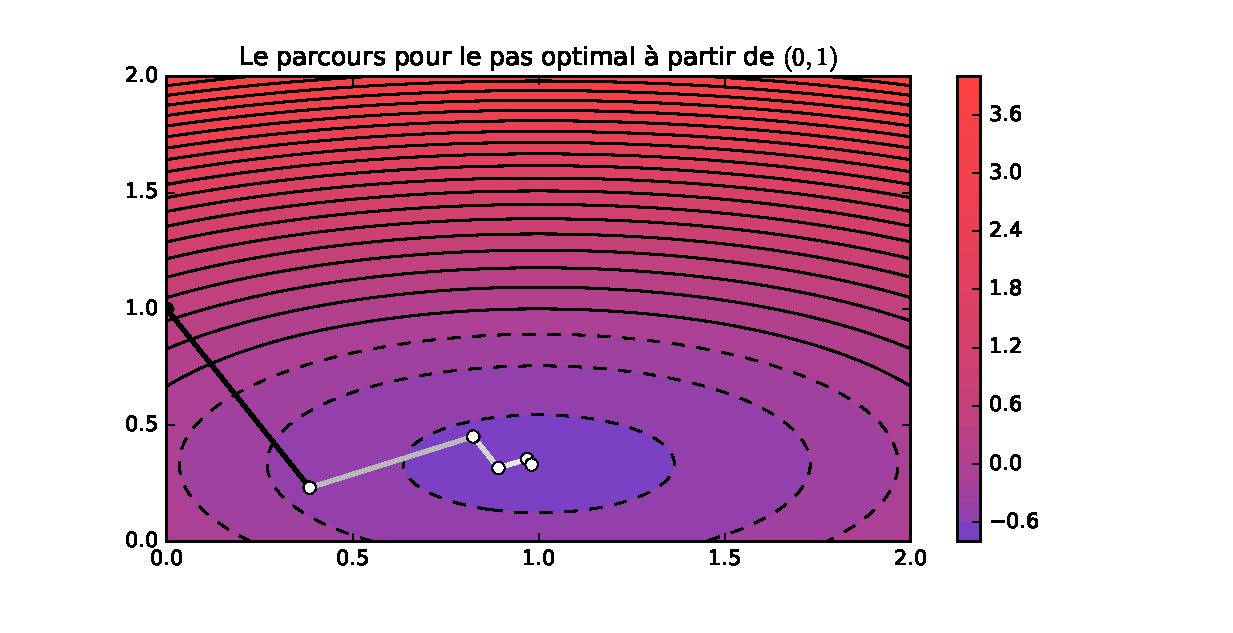
\includegraphics[height=8cm]{I123a.eps}
    \vspace{-1cm}
	\end{center}
	\caption{Parcours du méthode de gradient à pas optimal.}
	\label{fig:I23a}
\end{figure}
\begin{figure}[H]
	\begin{center}
\includegraphics[height=8cm]{I123b.eps}
    \vspace{-1cm}
	\end{center}
	\caption{Parcours du méthode de gradient à pas optimal.}
	\label{fig:I23b}
\end{figure}
	
\subsubsection
Quand on met en œuvre le procédé de dichotomie pour l'équation \ref{eq:rosenbrock}, on trouve le résultat ci-dessous.

\section{Méthodes newtoniennes}
\subsection{Méthode de Newton}
\subsection{Méthode de Gauss-Newton}
\subsubsection{}
On commence par calculer la matrice $Df(u)$ où $\left[Df(u)\right]_{ij} = \frac{\partial f_i(u)}{\partial u_j}$

\subsubsection{}

\subsubsection{}

\section{Application à l'équation de convection-diffusion}
\subsection{Différences schémas d'approximation}
\subsubsection{}
On remplace $u_i^n$ par $u(x_i, t_n)$ où $u$ est une fonction régulière. On commence par le développement de Taylor au tour du point $(x_i, t_n)$. Pour le schéma
\begin{align*}
\frac{u_i^{n+1}-u_i^{n}}{\Delta t} + a \frac{u_{i+1}^{n}-u_{i-1}^{n}}{2\Delta x} -b \frac{u_{i+1}^{n}-u_{i-1}^{n} - 2 u_i^{n}}{\Delta x^2} =0 \text{, on a}
\end{align*}
\begin{multline*}
u(x_{i \pm 1}, t_n)= u(x_{i}, t_{n}) \pm \Delta x \frac{\partial u}{\partial x} (x_{i}, t_{n}) + \frac{1}{2} \Delta x^2 \frac{\partial^2 u}{\partial x^2}(x_{i}, t_{n}) \pm \frac{1}{6} \Delta x^3 \frac{\partial^3 u}{\partial x^3}(x_{i}, t_{n}) \\ + \frac{1}{24} \Delta x^4 \frac{\partial^4 u}{\partial^4 x} (x_{i}, t_{n}) + \O (\Delta x^5) \text{,}
\end{multline*}
\begin{align*}
u(x_{i}, t_{n+1})=u(x_{i}, t_{n}) + \Delta t \frac{\partial u}{\partial t} (x_{i}, t_{n}) + \frac{1}{2} \Delta t^2 \frac{\partial^2 u}{\partial t^2} (x_{i}, t_{n}) + \O (\Delta t^3) \text{.}
\end{align*}
On remplace le développement dans l'erreur de troncature qui est définit comme
\begin{align*}
\begin{split}
E&=\frac{u_i^{n+1}-u_i^{n}}{\Delta t} + a \frac{u_{i+1}^{n}-u_{i-1}^{n}}{2\Delta x} -b \frac{u_{i+1}^{n}-u_{i-1}^{n} - 2 u_i^{n}}{\Delta x^2} \\
&= \frac{\partial u}{\partial t}(x_i, t_n) + a \frac{\partial u}{\partial x}(x_i, t_n) - b \frac{\partial^2 u}{\partial^2 t}(x_i, t_n) + \O (\Delta t + \Delta x^2)
\end{split}
\end{align*}
Le erreur ci-dessus est dans le "standard" mentionné dans le Remarque 2.2.5 du polycopié, c'est à dire, pour une fonction régulière qui n'est pas solution de notre problème, la limite de l'erreur de troncature n'est pas nulle. Alors c'est schéma est consistante et d'ordre 1 en temps et 2 en espace.
Pour le schéma
\begin{align*}
\frac{u_i^{n+1}-u_i^{n}}{\Delta t} + a \frac{u_{i+1}^{n+1}-u_{i-1}^{n+1}}{2\Delta x} -b \frac{u_{i+1}^{n+1}-u_{i-1}^{n+1} - 2 u_i^{n+1}}{\Delta x^2} =0 \text{,}
\end{align*}
on fait le développement au tour du point $(x_i, t_{n+1})$ et on trouve
\begin{multline*}
u(x_{i \pm 1}, t_{n+1})= u(x_{i}, t_{n+1}) \pm \Delta x \frac{\partial u}{\partial x} (x_{i}, t_{n+1}) + \frac{1}{2} \Delta x^2 \frac{\partial^2 u}{\partial x^2}(x_{i}, t_{n+1}) \pm \frac{1}{6} \Delta x^3 \frac{\partial^3 u}{\partial x^3}(x_{i}, t_{n+1}) \\ + \frac{1}{24} \Delta x^4 \frac{\partial^4 u}{\partial^4 x} (x_{i}, t_{n+1}) + \O (\Delta x^5) \text{,}
\end{multline*}
\begin{align*}
u(x_{i}, t_{n})=u(x_{i}, t_{n+1}) - \Delta t \frac{\partial u}{\partial t} (x_{i}, t_{n+1}) + \frac{1}{2} \Delta t^2 \frac{\partial^2 u}{\partial t^2} (x_{i}, t_{n+1}) + \O (\Delta t^3) \text{, et finalement}
\end{align*}

\begin{align*}
\begin{split}
E&=\frac{u_i^{n+1}-u_i^{n}}{\Delta t} + a \frac{u_{i+1}^{n+1}-u_{i-1}^{n+1}}{2\Delta x} -b \frac{u_{i+1}^{n+1}-u_{i-1}^{n+1} - 2 u_i^{n+1}}{\Delta x^2} \\
&= \frac{\partial u}{\partial t}(x_i, t_{n+1}) + a \frac{\partial u}{\partial x}(x_i, t_{n+1}) - b \frac{\partial^2 u}{\partial^2 t}(x_i, t_{n+1}) + \O (\Delta t + \Delta x^2) \text{.}
\end{split}
\end{align*}
Par le même argument du schéma antérieur, ce schéma est consistant d'ordre 1 en temps et 2 en espace.

\subsubsection
content...

\subsection{Schéma implicite}
\subsubsection{}
On peut récrire le schéma implicite comme
\begin{align*}
u_i^n= \left ( \frac{a \Delta t}{2 \Delta x} - \frac{b \Delta t}{\Delta x^2} \right ) u_{i+1}^{n+1} + \left ( 1 +  \frac{2 b \Delta t}{\Delta x^2} \right ) u_{i}^{n+1} + \left ( - \frac{a \Delta t}{2 \Delta x} - \frac{b \Delta t}{\Delta x^2} \right ) u_{i-1}^{n+1} \text{.}
\end{align*}
On pose
\begin{align*}
\gamma = \frac{a \Delta t}{2 \Delta x} \qquad \textrm{et} \qquad \delta=\frac{b \Delta t}{\Delta x^2} \text{.}
\end{align*}
Alors pour $U^n=MU^{n+1}$, où $U^n= \begin{pmatrix} u_{-i_\text{max}}^n \\ \vdots \\ u_{i_\text{max}}^n \end{pmatrix}$, on trouve
\begin{comment}
\begin{align*}
M=\begin{pmatrix} 
 1 + 2 \delta & \gamma - \delta & 0 & \dots  & 0 \\
 -\gamma - \delta & 1 + 2 \delta & \gamma - \delta & \dots  & 0 \\
 \vdots & -\gamma - \delta & \ddots & \ddots & \vdots \\
  0 & 0 & \ddots & 1 + 2 \delta  & \gamma - \delta \\
 0 & 0 & \dots & -\gamma - \delta &  1 + 2 \delta
\end{pmatrix}
\end{align*}
\end{comment}
$
M_{ij}=
\begin{cases}
1 + 2 \delta &\text{, si } i=j \\
\gamma - \delta  &\text{, si } i=j-1 \\
- \gamma - \delta &\text{, si } i=j+1 \\
0 &\text{, sinon}
\end{cases}
$.

\subsubsection{}
On définit $M^s =\frac{1}{2} (M + M^T) = M^s_{ij}=
\begin{cases}
1 + 2 \delta &\text{, si } i=j \\
- \delta &\text{, si } i =  j \pm 1 \\
0 &\text{, sinon}
\end{cases}
$. D'après \cite{weiss}, M est positive définit si et seulement si $M^s$ le est. D'après \cite{milica}, comme $\| 1 +2 \delta \| > \| - \delta \| + \| - \delta \|$, $M^s$ est définit positive, alors $M$ est définit positive. Ce qu'implique que $M$ est inversible.

\subsubsection{}
content...
\section{Application à l'équation de la chaleur non linéaire}
\subsection{Schéma implicite linéaire}

\subsubsection{}
content...

\subsubsection{}
content...

\subsection{Schéma pour l'équation stationnaire}
\subsubsection{}
content...

\subsubsection{}
content...

\begin{thebibliography}{3}

	\bibitem{weiss} 
	Weisstein, Eric W.
	\textit{Positive Definite Matrices}. 
	From MathWorld--A Wolfram Web Resource. \url{http://mathworld.wolfram.com/PositiveDefiniteMatrix.html}
	
    \bibitem{milica} 
	Milica Anđelić and C. M. da Fonseca.
	\textit{Sufficient Conditions for Positive Definiteness of Tridiagonal Matricies Revisited}.
   \url{http://www.mat.uc.pt/~cmf/papers/tri_positive_definite_revisited.pdf}
    
\end{thebibliography}
\end{document}